\documentclass[12pt,a4paper]{report}

% ---------- Packages ----------
\usepackage[margin=1in]{geometry}
\usepackage{graphicx}
\usepackage{tikz}
\usetikzlibrary{shapes.geometric,shapes.multipart,arrows.meta,positioning,shapes.symbols,calc,fit,backgrounds}
\usepackage{array}
\usepackage{longtable}
\usepackage{booktabs}
\usepackage{enumitem}
\usepackage{titlesec}
\usepackage{hyperref}
\usepackage{xcolor}
\usepackage{fancyhdr}
\usepackage{parskip}
\usepackage{caption}

\hypersetup{
    colorlinks=true,
    linkcolor=black,
    urlcolor=blue,
    citecolor=black,
    pdftitle={PromptBench - Software Engineering Project Report},
}

\pagestyle{fancy}
\fancyhf{}
\fancyhead[R]{\small PromptBench}
\fancyhead[L]{\small UCS 318 Software Engineering Project Report}
\fancyfoot[C]{\thepage}
\renewcommand{\headrulewidth}{0.4pt}

\titleformat{\chapter}[hang]{\normalfont\huge\bfseries}{\thechapter.}{1em}{}
\titlespacing*{\chapter}{0pt}{-20pt}{20pt}

% ---------- Stick-figure actor macro for UML use-case diagrams ----------
\newcommand{\stickactor}[2]{%
  \begin{scope}[shift={(#1)}]
    \draw[thick] (0,1.55) circle (0.22);
    \draw[thick] (0,1.33) -- (0,0.55);
    \draw[thick] (-0.35,1.05) -- (0.35,1.05);
    \draw[thick] (0,0.55) -- (-0.3,0.0);
    \draw[thick] (0,0.55) -- (0.3,0.0);
    \node[align=center,font=\small] at (0,-0.35) {#2};
  \end{scope}
}

\begin{document}

% ======================================================
% TITLE PAGE
% ======================================================
\begin{titlepage}
\centering
\vspace*{0.5cm}

{\Huge \textbf{PromptBench}}\\[0.3cm]
{\large \textit{Practice AI-Collaboration Skills Through Graded Business Case Studies}}\\[1cm]

{\large \textbf{UCS 318 Software Engineering Project Report -- Semester Evaluation}}\\[1.5cm]

{\textbf{Submitted by:}}\\[0.3cm]
Ridham Goyal (1024030417)\\[0.2cm]
Niloy Sharma (1024030422)\\[1.5cm]

{\textbf{Submitted to:}}\\[0.3cm]
\rule{6cm}{0.4pt}\\[2cm]

\vfill


\includegraphics[width=0.22\textwidth]{images/logo-000.png}\\[0.3cm]
{\large \textbf{THAPAR INSTITUTE OF ENGINEERING \& TECHNOLOGY}}\\
{\small (Deemed to be University)}\\[1cm]

{\textbf{Computer Science and Engineering Department}}\\
{\textbf{TIET, Patiala}}

\end{titlepage}

% ======================================================
% ACKNOWLEDGEMENT
% ======================================================
\chapter*{Acknowledgement}
\addcontentsline{toc}{chapter}{Acknowledgement}

We take this opportunity to express our sincere gratitude to everyone who contributed to the
successful completion of our project ``PromptBench.''

First and foremost, we would like to extend our heartfelt thanks to our project supervisor for
continuous guidance, valuable suggestions, and constructive feedback throughout the duration of
our project. This encouragement and expertise played a pivotal role in helping us understand the
technical challenges and refine our approach at every stage.

We are also grateful to the Thapar Institute of Engineering and Technology (TIET) for providing
us with the necessary resources, infrastructure, and learning environment required to develop
this project effectively. Their support enabled us to explore, design, and build a fully
functioning full-stack system with confidence. Our sincere thanks also go to our peers and
classmates for their insightful discussions, suggestions, and motivation during the development
of this work. Their input helped us improve several aspects of the project, both technically and
conceptually. Lastly, we would like to express our deep appreciation to our families for their
constant encouragement, patience, and belief in us. Their support has been a source of
inspiration throughout the journey.

We wholeheartedly dedicate this project to everyone who supported us, guided us, and stood by us
in completing PromptBench successfully.

\vspace{1cm}

\begin{center}
\begin{tabular}{|c|l|c|}
\hline
\textbf{S.No.} & \textbf{Student Name} & \textbf{Roll Number} \\
\hline
1 & Ridham Goyal & 1024030417 \\
\hline
2 & Niloy Sharma & 1024030422 \\
\hline
\end{tabular}
\end{center}

\tableofcontents

% ======================================================
\chapter{Project Selection Phase}
% ======================================================

In this phase, the final project idea is chosen based on feasibility, requirements, and expected
outcomes. This provides a clear foundation for preparing the software bid.

\section{Software Bid}

\textbf{Programming Language / Environment Experience}\\
The languages and frameworks the team is most comfortable developing in, used across the project,
in order of preference:
\begin{enumerate}[nosep]
    \item Python (FastAPI, SQLAlchemy, Pydantic)
    \item JavaScript / JSX (React, Vite)
    \item SQL (PostgreSQL)
\end{enumerate}

\textbf{Choices of Projects}

\begin{center}
\renewcommand{\arraystretch}{1.5}
\begin{tabular}{|p{2.3cm}|p{3.2cm}|p{8.5cm}|}
\hline
\textbf{} & \textbf{Project Name} & \textbf{Unique Selling Point} \\
\hline
First Choice & PromptBench & A benchmarking platform that evaluates how well a candidate
\emph{collaborates} with an AI assistant to solve open-ended business case studies, rather than
testing raw coding ability. A strict Helper-AI/Judge-AI isolation boundary ensures the grading
rubric and ground truth are never exposed to the candidate-facing assistant, keeping evaluations
fair and tamper-resistant. \\
\hline
\end{tabular}
\end{center}

\textbf{Additional Remarks / Inputs}

The development of PromptBench provided valuable insights into real-world full-stack software
development, LLM-integration patterns, and secure system design. Challenges were faced while
designing the Helper/Judge isolation boundary, structuring the anti-gaming heuristics, and
enforcing a strict JSON schema on LLM-generated evaluation output. In the future, the system can
be enhanced with additional case categories, richer analytics dashboards, and organisation-level
reporting for recruiters. Overall, this project serves as a strong foundation for a
skills-based, AI-native assessment platform.

\section{Project Overview}

\textbf{Purpose}\\
The main goal of PromptBench is to:
\begin{itemize}[nosep]
    \item Give candidates a realistic environment to practice using an AI assistant to solve
    open-ended business problems.
    \item Evaluate collaboration skills -- clarifying questions, iterative refinement, and
    hallucination-catching -- rather than just the final answer.
    \item Produce transparent, rubric-grounded feedback that candidates can learn from.
    \item Protect the integrity of the evaluation by isolating grading logic from the
    candidate-facing assistant.
\end{itemize}

\textbf{Target Users}
\begin{itemize}[nosep]
    \item \textbf{Candidates} -- practice solving business case studies with an AI assistant and
    receive a graded evaluation.
    \item \textbf{Helper AI} -- a conversational assistant available to the candidate during the
    exercise.
    \item \textbf{Judge AI} -- a server-side evaluator invoked only at final submission time.
\end{itemize}

\textbf{Key Features}
\begin{itemize}[nosep]
    \item Secure signup / login (bcrypt password hashing + JWT sessions)
    \item Browsable library of business case studies (data diagnosis, strategy generation,
    customer reasoning categories, at easy/medium/hard difficulty)
    \item Interactive case workspace with a Helper AI chat assistant
    \item Final-answer submission with automated rubric-based grading
    \item Anti-gaming heuristics (near-zero conversation, too-fast submission, pre-written answer
    detection)
    \item Score dashboard with 4-dimension breakdown and judge reasoning
    \item Attempt history so candidates can track improvement over time
\end{itemize}

\textbf{System Overview}\\
PromptBench operates as a web-based platform where:
\begin{enumerate}[nosep]
    \item Candidates create accounts and log in.
    \item Candidates browse the five seeded case studies and start an attempt.
    \item Candidates converse with the Helper AI, which only ever sees the public case context.
    \item Candidates draft and submit a final written recommendation.
    \item The backend runs anti-gaming checks and then invokes the Judge AI, which independently
    sees the rubric, hidden ground-truth notes, the full transcript, and the final answer.
    \item Candidates receive a structured score (0--100), four dimension sub-scores, judge
    reasoning, and any anti-gaming flags, and can revisit this history at any time.
\end{enumerate}

% ======================================================
\chapter{Analysis Phase}
% ======================================================

\section{Use Case}

\textbf{Actors}
\begin{itemize}[nosep]
    \item Candidate
    \item Helper AI (candidate-facing assistant)
    \item Judge AI (server-side evaluator)
\end{itemize}

\textbf{Candidate Use Cases}
\begin{enumerate}[nosep]
    \item Sign Up / Log In
    \item Browse Case Studies
    \item Start Case Attempt
    \item Chat with Helper AI
    \item Draft \& Submit Final Answer
    \item View Evaluation Report
    \item View Attempt History
\end{enumerate}

\textbf{Helper AI Use Case}
\begin{enumerate}[nosep,start=8]
    \item Generate Contextual Response
\end{enumerate}

\textbf{Judge AI Use Cases}
\begin{enumerate}[nosep,start=9]
    \item Run Anti-Gaming Checks
    \item Evaluate Transcript \& Final Answer Against Rubric
\end{enumerate}

\subsection{Use-Case Diagram}

The Use Case Diagram of PromptBench illustrates the interactions between the Candidate, the
Helper AI, and the Judge AI. The candidate signs up/logs in, browses case studies, starts an
attempt, chats with the Helper AI, and submits a final answer. Submitting a final answer always
\emph{includes} running anti-gaming checks and invoking the Judge AI evaluation, after which the
candidate can view the evaluation report and their attempt history. The diagram uses
\texttt{<<include>>} and \texttt{<<extend>>} relationships to show mandatory and optional
dependencies between use cases.

\begin{center}
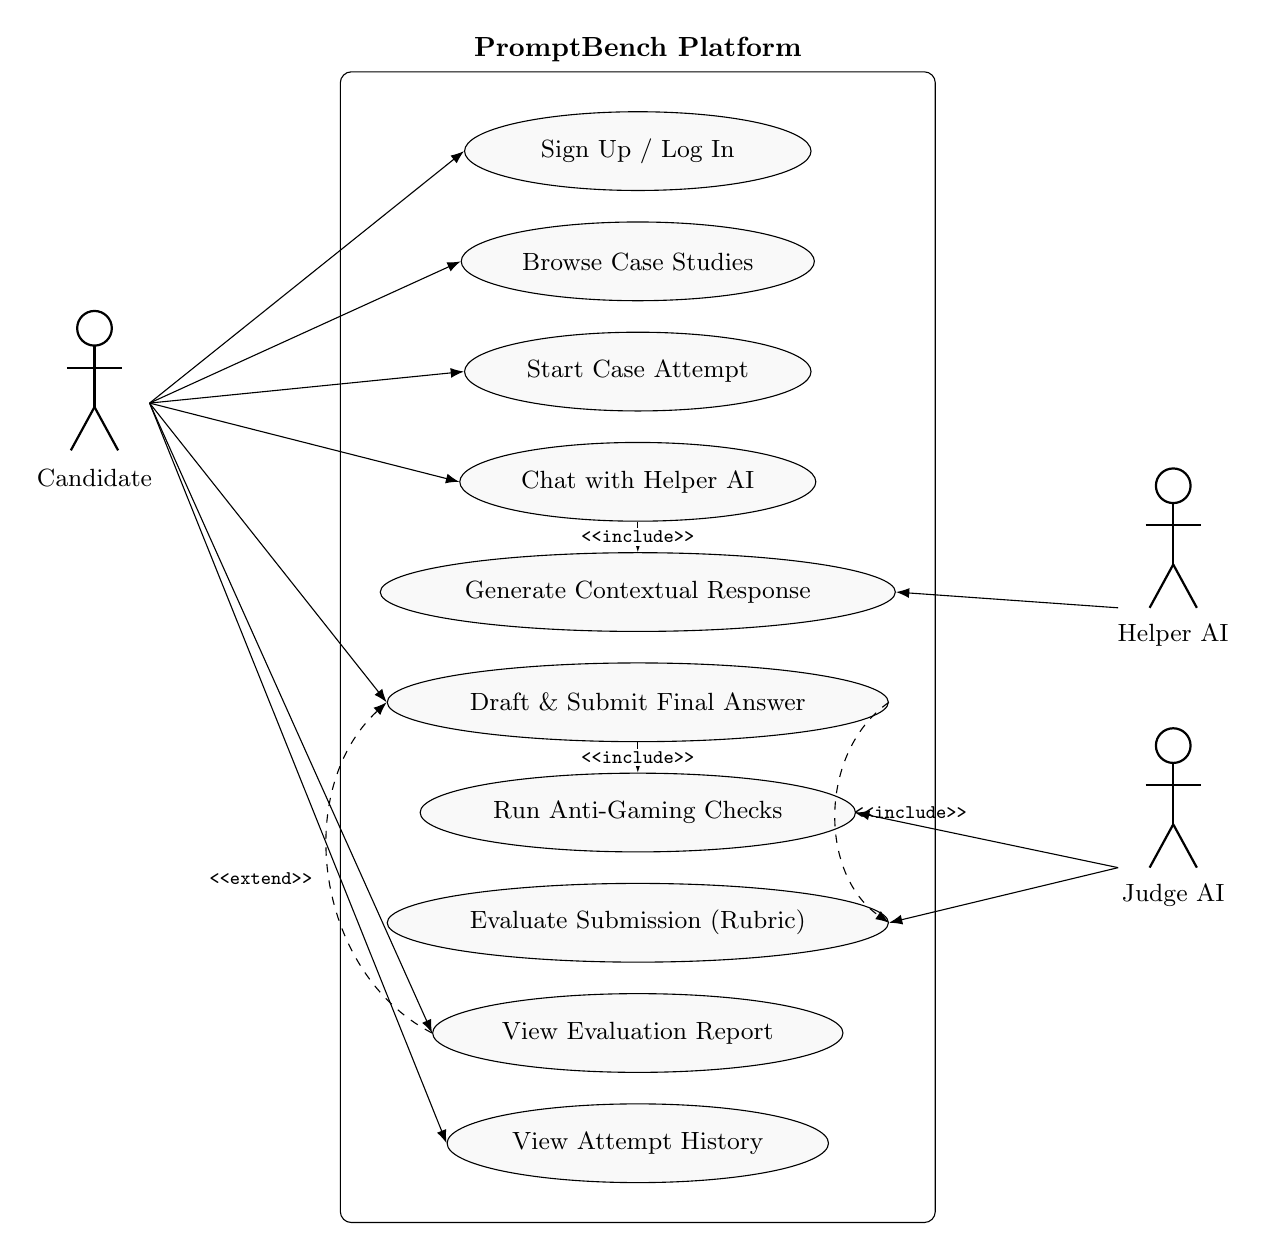
\begin{tikzpicture}[
    usecase/.style={ellipse, draw, minimum width=4.4cm, minimum height=1.0cm, align=center, font=\small, fill=gray!5},
    yscale=1
]
    \node[usecase] (uc1)  at (4.6,8.4)  {Sign Up / Log In};
    \node[usecase] (uc2)  at (4.6,7.0)  {Browse Case Studies};
    \node[usecase] (uc3)  at (4.6,5.6)  {Start Case Attempt};
    \node[usecase] (uc4)  at (4.6,4.2)  {Chat with Helper AI};
    \node[usecase] (uc10) at (4.6,2.8)  {Generate Contextual Response};
    \node[usecase] (uc5)  at (4.6,1.4)  {Draft \& Submit Final Answer};
    \node[usecase] (uc6)  at (4.6,0.0)  {Run Anti-Gaming Checks};
    \node[usecase] (uc7)  at (4.6,-1.4) {Evaluate Submission (Rubric)};
    \node[usecase] (uc8)  at (4.6,-2.8) {View Evaluation Report};
    \node[usecase] (uc9)  at (4.6,-4.2) {View Attempt History};

    \begin{scope}[on background layer]
    \node[draw, rounded corners, fit=(uc1)(uc2)(uc3)(uc4)(uc10)(uc5)(uc6)(uc7)(uc8)(uc9), inner sep=0.5cm, label={[font=\bfseries]above:PromptBench Platform}] (sys) {};
    \end{scope}

    \stickactor{-2.3,4.6}{Candidate}
    \stickactor{11.4,-0.7}{Judge AI}
    \stickactor{11.4,2.6}{Helper AI}

    \draw[-{Latex}] (-1.6,5.2) -- (uc1.west);
    \draw[-{Latex}] (-1.6,5.2) -- (uc2.west);
    \draw[-{Latex}] (-1.6,5.2) -- (uc3.west);
    \draw[-{Latex}] (-1.6,5.2) -- (uc4.west);
    \draw[-{Latex}] (-1.6,5.2) -- (uc5.west);
    \draw[-{Latex}] (-1.6,5.2) -- (uc8.west);
    \draw[-{Latex}] (-1.6,5.2) -- (uc9.west);

    \draw[dashed,-{Latex}] (uc4) -- (uc10) node[midway,fill=white,inner sep=1pt,font=\scriptsize] {\texttt{<<include>>}};
    \draw[dashed,-{Latex}] (uc5) -- (uc6) node[midway,fill=white,inner sep=1pt,font=\scriptsize] {\texttt{<<include>>}};
    \draw[dashed,-{Latex}] (uc5.east) to[bend right=55] node[pos=0.5,right=0.1cm,font=\scriptsize] {\texttt{<<include>>}} (uc7.east);
    \draw[dashed,-{Latex}] (uc8.west) to[bend left=55] node[pos=0.5,left=0.1cm,font=\scriptsize] {\texttt{<<extend>>}} (uc5.west);

    \draw[-{Latex}] (10.7,-0.7) -- (uc6.east);
    \draw[-{Latex}] (10.7,-0.7) -- (uc7.east);
    \draw[-{Latex}] (10.7,2.6) -- (uc10.east);
\end{tikzpicture}
\end{center}

\subsection{Use-Case Templates}

\textbf{Use Case: Chat with Helper AI}\\
\emph{Actor:} Candidate\\
\emph{Description:} Candidate exchanges messages with the Helper AI while working on a case.\\
\emph{Preconditions:} A case attempt has been started.\\
\emph{Postconditions:} A new pair of transcript turns (candidate + assistant) is persisted.\\
\emph{Main Flow:}
\begin{enumerate}[nosep]
    \item Candidate sends a message.
    \item System stores the candidate's turn and loads the full conversation history.
    \item System calls the Helper AI with the case context and history.
    \item Helper AI's reply is stored and returned to the candidate.
\end{enumerate}
\emph{Relationship:} Includes $\rightarrow$ Generate Contextual Response

\vspace{0.3cm}
\textbf{Use Case: Draft \& Submit Final Answer}\\
\emph{Actor:} Candidate\\
\emph{Description:} Candidate submits a final written recommendation for grading.\\
\emph{Preconditions:} Submission status is \texttt{in\_progress} or \texttt{evaluation\_failed}.\\
\emph{Postconditions:} Submission status becomes \texttt{submitted} and an Evaluation record is created.\\
\emph{Main Flow:}
\begin{enumerate}[nosep]
    \item Candidate submits final answer text.
    \item System timestamps the submission and loads the full transcript.
    \item System runs anti-gaming checks on timing and transcript content.
    \item System invokes the Judge AI with rubric, ground truth, transcript, and final answer.
    \item System validates the Judge's JSON response against a strict schema and persists the Evaluation.
\end{enumerate}
\emph{Relationship:} Includes $\rightarrow$ Run Anti-Gaming Checks, Evaluate Submission (Rubric)

\vspace{0.3cm}
\textbf{Use Case: Run Anti-Gaming Checks}\\
\emph{Actor:} Judge AI (system)\\
\emph{Description:} System flags suspicious submission patterns before/alongside grading.\\
\emph{Preconditions:} Final answer has been submitted.\\
\emph{Postconditions:} A list of flags (possibly empty) is attached to the evaluation.\\
\emph{Main Flow:}
\begin{enumerate}[nosep]
    \item Check whether the transcript has fewer than 2 turns (near-zero conversation).
    \item Check whether the elapsed time between \texttt{started\_at} and \texttt{submitted\_at} is under 30 seconds.
    \item Check whether the first candidate message is highly similar (Jaccard $\geq 0.5$) to the final answer and over 500 characters (pre-written answer).
\end{enumerate}

\vspace{0.3cm}
\textbf{Use Case: Evaluate Submission (Rubric)}\\
\emph{Actor:} Judge AI\\
\emph{Description:} Judge AI grades the transcript and final answer against the hidden rubric.\\
\emph{Preconditions:} Anti-gaming checks have completed.\\
\emph{Postconditions:} An overall score, four dimension scores, and reasoning are produced.\\
\emph{Main Flow:}
\begin{enumerate}[nosep]
    \item System formats the rubric, ground-truth notes, transcript, and final answer into a prompt.
    \item Judge LLM returns a JSON grading report.
    \item System parses and validates the JSON against a strict Pydantic schema, retrying extraction if the response is wrapped in extra text.
\end{enumerate}

\vspace{0.3cm}
\textbf{Use Case: View Evaluation Report / Attempt History}\\
\emph{Actor:} Candidate\\
\emph{Description:} Candidate reviews the score dashboard for a submission, or the list of all past graded attempts.\\
\emph{Preconditions:} At least one submission has status \texttt{submitted}.\\
\emph{Postconditions:} Score, dimension breakdown, judge reasoning, and anti-gaming flags are displayed.

\section{Activity Diagram and Swimlane Diagram}

The Activity Diagram illustrates the complete workflow of PromptBench: a candidate authenticates,
starts a case, iterates with the Helper AI, and submits a final answer, which triggers anti-gaming
checks and Judge AI grading before results are shown back to the candidate.

\begin{center}
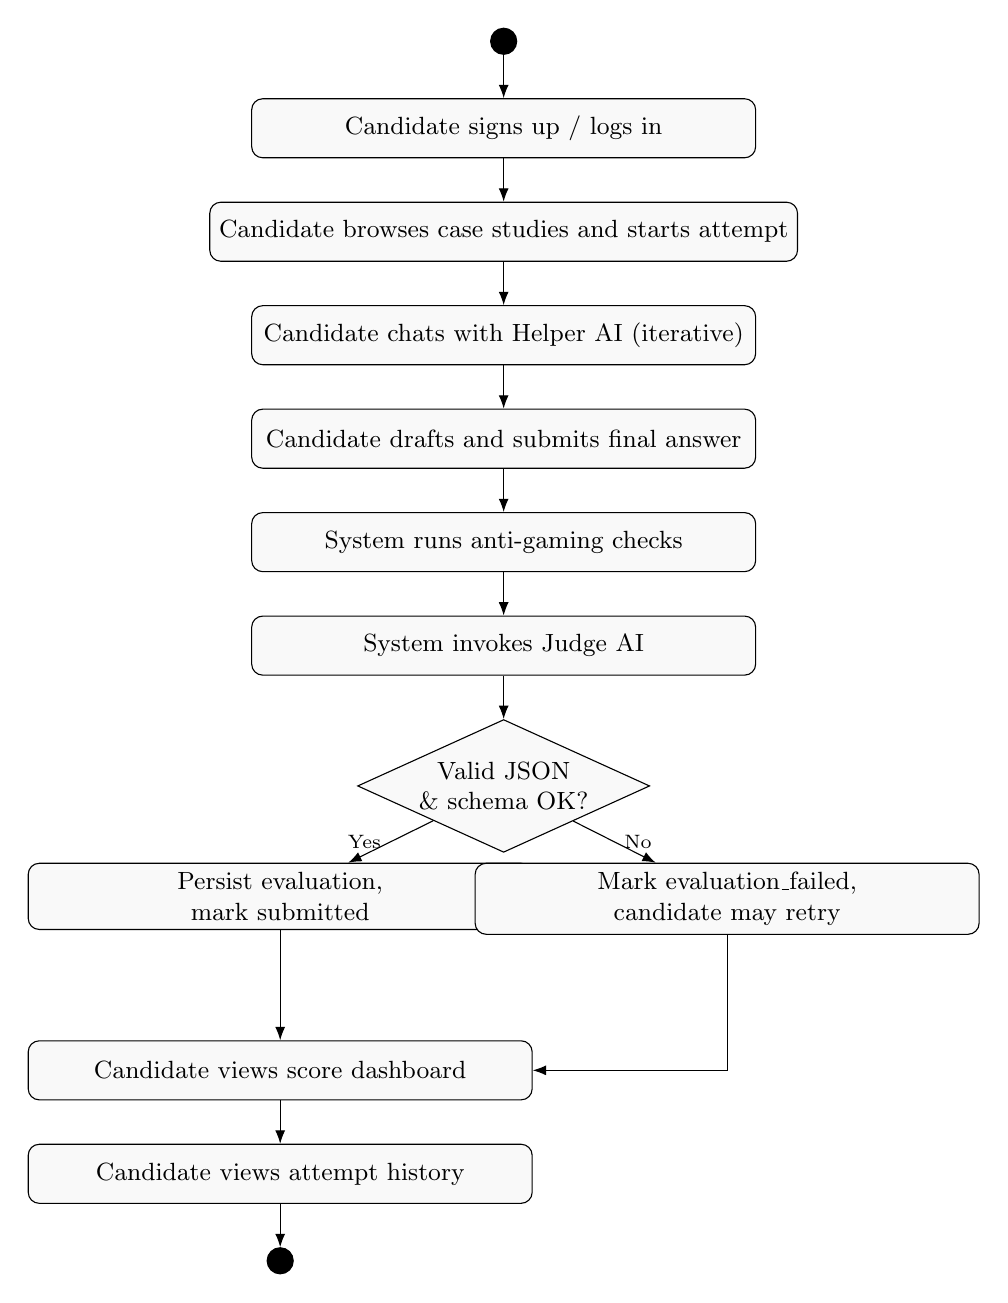
\begin{tikzpicture}[
    node distance=0.55cm and 1.2cm,
    act/.style={draw, rounded corners, minimum width=6.4cm, minimum height=0.75cm, align=center, font=\small, fill=gray!5},
    dec/.style={draw, diamond, aspect=2.2, align=center, font=\small, fill=gray!5, inner sep=1pt},
    start/.style={draw, circle, fill=black, minimum size=0.25cm},
    stop/.style={draw, circle, fill=black, minimum size=0.25cm}
]
\node[start] (s0) {};
\node[act, below=of s0] (a1) {Candidate signs up / logs in};
\node[act, below=of a1] (a2) {Candidate browses case studies and starts attempt};
\node[act, below=of a2] (a3) {Candidate chats with Helper AI (iterative)};
\node[act, below=of a3] (a4) {Candidate drafts and submits final answer};
\node[act, below=of a4] (a5) {System runs anti-gaming checks};
\node[act, below=of a5] (a6) {System invokes Judge AI};
\node[dec, below=of a6] (d1) {Valid JSON \\ \& schema OK?};
\node[act, below left=0.55cm and -1.3cm of d1] (a7) {Persist evaluation,\\ mark submitted};
\node[act, below right=0.55cm and -1.3cm of d1] (a8) {Mark evaluation\_failed,\\ candidate may retry};
\node[act, below=1.4cm of a7] (a9) {Candidate views score dashboard};
\node[act, below=of a9] (a10) {Candidate views attempt history};
\node[stop, below=of a10] (s1) {};

\draw[-{Latex}] (s0) -- (a1);
\draw[-{Latex}] (a1) -- (a2);
\draw[-{Latex}] (a2) -- (a3);
\draw[-{Latex}] (a3) -- (a4);
\draw[-{Latex}] (a4) -- (a5);
\draw[-{Latex}] (a5) -- (a6);
\draw[-{Latex}] (a6) -- (d1);
\draw[-{Latex}] (d1) -- node[left,font=\scriptsize]{Yes} (a7);
\draw[-{Latex}] (d1) -- node[right,font=\scriptsize]{No} (a8);
\draw[-{Latex}] (a7) -- (a9);
\draw[-{Latex}] (a8) |- (a9.east);
\draw[-{Latex}] (a9) -- (a10);
\draw[-{Latex}] (a10) -- (s1);
\end{tikzpicture}
\end{center}

This swimlane diagram highlights the same workflow split across the four responsible
participants: Candidate, Backend System, Helper AI, and Judge AI.

\begin{center}
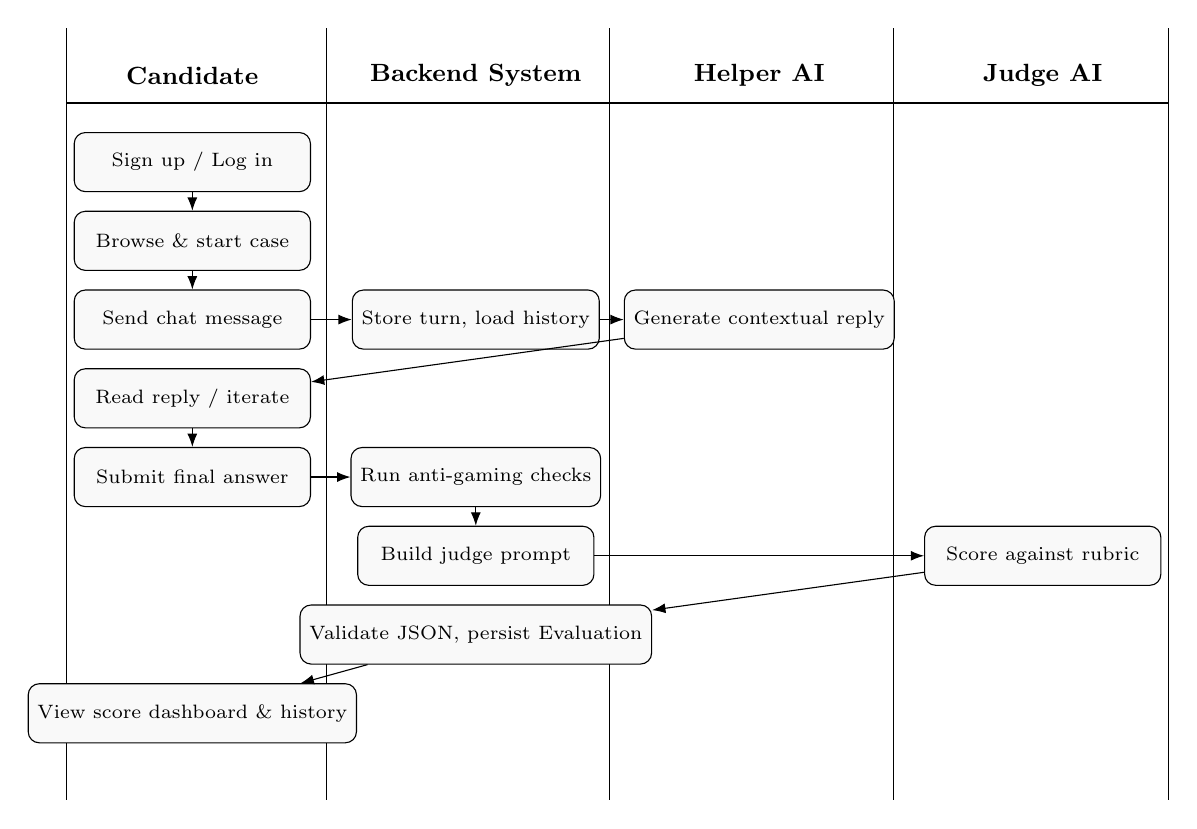
\begin{tikzpicture}[
    node distance=0.5cm and 0.4cm,
    act/.style={draw, rounded corners, minimum width=3.0cm, minimum height=0.75cm, align=center, font=\scriptsize, fill=gray!5}
]
    % Lane headers
    \node[font=\bfseries\small] (h1) at (0,0) {Candidate};
    \node[font=\bfseries\small] (h2) at (3.6,0) {Backend System};
    \node[font=\bfseries\small] (h3) at (7.2,0) {Helper AI};
    \node[font=\bfseries\small] (h4) at (10.8,0) {Judge AI};

    \draw (-1.6,-0.35) -- (12.4,-0.35);
    \draw (1.7,0.6) -- (1.7,-9.2);
    \draw (5.3,0.6) -- (5.3,-9.2);
    \draw (8.9,0.6) -- (8.9,-9.2);
    \draw (-1.6,0.6) -- (-1.6,-9.2);
    \draw (12.4,0.6) -- (12.4,-9.2);

    \node[act] (c1) at (0,-1.1) {Sign up / Log in};
    \node[act] (c2) at (0,-2.1) {Browse \& start case};
    \node[act] (c3) at (0,-3.1) {Send chat message};
    \node[act] (b3) at (3.6,-3.1) {Store turn, load history};
    \node[act] (h1b) at (7.2,-3.1) {Generate contextual reply};
    \node[act] (c4) at (0,-4.1) {Read reply / iterate};
    \node[act] (c5) at (0,-5.1) {Submit final answer};
    \node[act] (b5) at (3.6,-5.1) {Run anti-gaming checks};
    \node[act] (b6) at (3.6,-6.1) {Build judge prompt};
    \node[act] (j1) at (10.8,-6.1) {Score against rubric};
    \node[act] (b7) at (3.6,-7.1) {Validate JSON, persist Evaluation};
    \node[act] (c6) at (0,-8.1) {View score dashboard \& history};

    \draw[-{Latex}] (c1) -- (c2);
    \draw[-{Latex}] (c2) -- (c3);
    \draw[-{Latex}] (c3) -- (b3);
    \draw[-{Latex}] (b3) -- (h1b);
    \draw[-{Latex}] (h1b) -- (c4);
    \draw[-{Latex}] (c4) -- (c5);
    \draw[-{Latex}] (c5) -- (b5);
    \draw[-{Latex}] (b5) -- (b6);
    \draw[-{Latex}] (b6) -- (j1);
    \draw[-{Latex}] (j1) -- (b7);
    \draw[-{Latex}] (b7) -- (c6);
\end{tikzpicture}
\end{center}

\section{Data Flow Diagrams (DFDs)}

The following figures illustrate the flow of information within PromptBench, from a high-level
context down to detailed process-level data movement.

\subsection{DFD Level 0}

The Level 0 DFD provides a context-level overview: the Candidate exchanges case data, chat
messages, and final answers with the PromptBench System, and the system in turn calls out to the
Anthropic API (LLM provider) to power both the Helper AI and the Judge AI.

\begin{center}
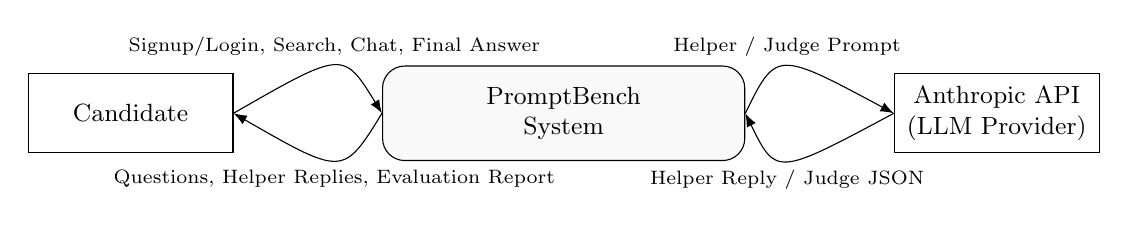
\begin{tikzpicture}[
    ext/.style={draw, minimum width=2.6cm, minimum height=1.0cm, align=center, font=\small},
    proc/.style={draw, rounded corners=8pt, minimum width=4.6cm, minimum height=1.2cm, align=center, font=\small, fill=gray!5}
]
    \node[ext] (cand) at (0,0) {Candidate};
    \node[proc] (sys) at (5.5,0) {PromptBench\\System};
    \node[ext] (llm) at (11,0) {Anthropic API\\(LLM Provider)};

    \draw[-{Latex}] (cand.east) .. controls (2.7,0.8) .. (sys.west) node[midway,above,font=\scriptsize] {Signup/Login, Search, Chat, Final Answer};
    \draw[-{Latex}] (sys.west) .. controls (2.7,-0.8) .. (cand.east) node[midway,below,font=\scriptsize] {Questions, Helper Replies, Evaluation Report};

    \draw[-{Latex}] (sys.east) .. controls (8.2,0.8) .. (llm.west) node[midway,above,font=\scriptsize] {Helper / Judge Prompt};
    \draw[-{Latex}] (llm.west) .. controls (8.2,-0.8) .. (sys.east) node[midway,below,font=\scriptsize] {Helper Reply / Judge JSON};
\end{tikzpicture}
\end{center}

\subsection{DFD Level 1}

The Level 1 DFD breaks the system into its five core processes and four data stores.

\begin{center}
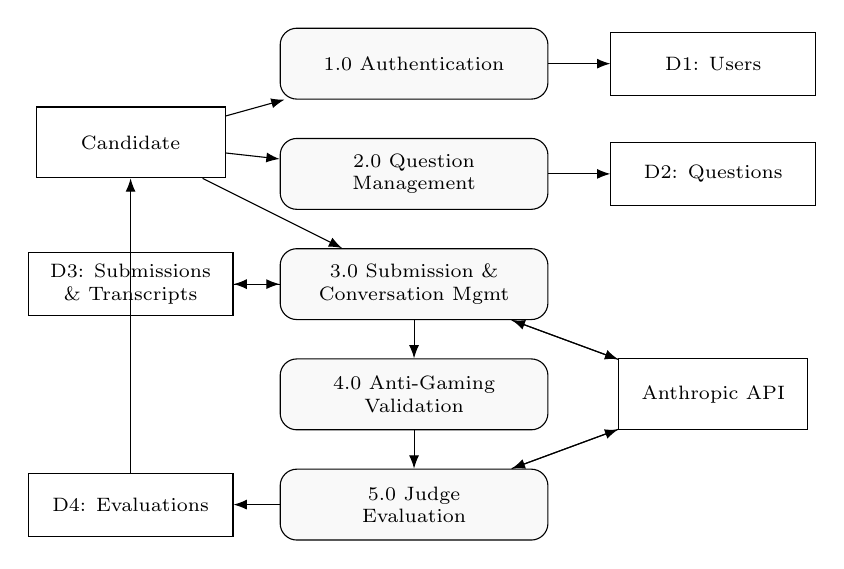
\begin{tikzpicture}[
    ext/.style={draw, minimum width=2.4cm, minimum height=0.9cm, align=center, font=\scriptsize},
    proc/.style={draw, rounded corners=6pt, minimum width=3.4cm, minimum height=0.9cm, align=center, font=\scriptsize, fill=gray!5},
    store/.style={draw, minimum width=2.6cm, minimum height=0.8cm, align=center, font=\scriptsize, path picture={
        \draw ([xshift=0pt]path picture bounding box.north west) -- ([xshift=0pt]path picture bounding box.south west);
    }}
]
    \node[ext] (cand) at (0,2.4) {Candidate};
    \node[proc] (p1) at (3.6,3.4) {1.0 Authentication};
    \node[proc] (p2) at (3.6,2.0) {2.0 Question\\Management};
    \node[proc] (p3) at (3.6,0.6) {3.0 Submission \&\\Conversation Mgmt};
    \node[proc] (p4) at (3.6,-0.8) {4.0 Anti-Gaming\\Validation};
    \node[proc] (p5) at (3.6,-2.2) {5.0 Judge\\Evaluation};
    \node[ext] (llm) at (7.4,-0.8) {Anthropic API};

    \node[store] (d1) at (7.4,3.4) {D1: Users};
    \node[store] (d2) at (7.4,2.0) {D2: Questions};
    \node[store] (d3) at (0,0.6) {D3: Submissions\\\& Transcripts};
    \node[store] (d4) at (0,-2.2) {D4: Evaluations};

    \draw[-{Latex}] (cand) -- (p1);
    \draw[-{Latex}] (p1) -- (d1);
    \draw[-{Latex}] (cand) -- (p2);
    \draw[-{Latex}] (p2) -- (d2);
    \draw[-{Latex}] (cand) -- (p3);
    \draw[-{Latex}] (p3) -- (d3);
    \draw[-{Latex}] (d3) -- (p3);
    \draw[-{Latex}] (p3) -- (llm);
    \draw[-{Latex}] (llm) -- (p3);
    \draw[-{Latex}] (p3) -- (p4);
    \draw[-{Latex}] (p4) -- (p5);
    \draw[-{Latex}] (p5) -- (llm);
    \draw[-{Latex}] (llm) -- (p5);
    \draw[-{Latex}] (p5) -- (d4);
    \draw[-{Latex}] (d4) -- (cand);
\end{tikzpicture}
\end{center}

\subsection{DFD Level 2}

The Level 2 DFD expands processes 3.0 and 5.0, mirroring the actual backend logic in
\texttt{submissions.py}, \texttt{anti\_gaming.py}, and \texttt{judge\_llm.py}.

\begin{center}
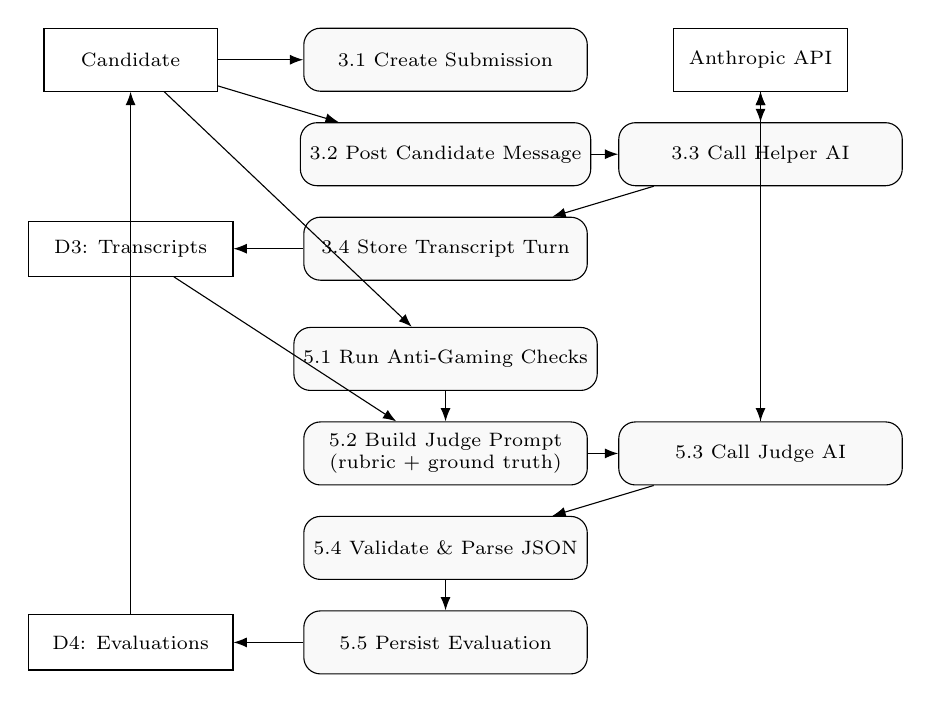
\begin{tikzpicture}[
    proc/.style={draw, rounded corners=6pt, minimum width=3.6cm, minimum height=0.8cm, align=center, font=\scriptsize, fill=gray!5},
    ext/.style={draw, minimum width=2.2cm, minimum height=0.8cm, align=center, font=\scriptsize},
    store/.style={draw, minimum width=2.6cm, minimum height=0.7cm, align=center, font=\scriptsize}
]
    \node[ext] (cand) at (0,3.2) {Candidate};
    \node[proc] (p31) at (4,3.2) {3.1 Create Submission};
    \node[proc] (p32) at (4,2.0) {3.2 Post Candidate Message};
    \node[proc] (p33) at (8,2.0) {3.3 Call Helper AI};
    \node[proc] (p34) at (4,0.8) {3.4 Store Transcript Turn};
    \node[store] (d3) at (0,0.8) {D3: Transcripts};

    \node[proc] (p51) at (4,-0.6) {5.1 Run Anti-Gaming Checks};
    \node[proc] (p52) at (4,-1.8) {5.2 Build Judge Prompt\\(rubric + ground truth)};
    \node[proc] (p53) at (8,-1.8) {5.3 Call Judge AI};
    \node[proc] (p54) at (4,-3.0) {5.4 Validate \& Parse JSON};
    \node[proc] (p55) at (4,-4.2) {5.5 Persist Evaluation};
    \node[store] (d4) at (0,-4.2) {D4: Evaluations};
    \node[ext] (llm) at (8,3.2) {Anthropic API};

    \draw[-{Latex}] (cand) -- (p31);
    \draw[-{Latex}] (cand) -- (p32);
    \draw[-{Latex}] (p32) -- (p33);
    \draw[-{Latex}] (p33) -- (llm);
    \draw[-{Latex}] (llm) -- (p33);
    \draw[-{Latex}] (p33) -- (p34);
    \draw[-{Latex}] (p34) -- (d3);
    \draw[-{Latex}] (d3) -- (p52);

    \draw[-{Latex}] (cand) -- (p51);
    \draw[-{Latex}] (p51) -- (p52);
    \draw[-{Latex}] (p52) -- (p53);
    \draw[-{Latex}] (p53) -- (llm);
    \draw[-{Latex}] (llm) -- (p53);
    \draw[-{Latex}] (p53) -- (p54);
    \draw[-{Latex}] (p54) -- (p55);
    \draw[-{Latex}] (p55) -- (d4);
    \draw[-{Latex}] (d4) -- (cand);
\end{tikzpicture}
\end{center}

\section{Software Requirement Specification (IEEE Format)}

\subsection{Introduction}

\subsubsection{Purpose}
The purpose of this document is to provide a detailed description of PromptBench, a platform
designed to let candidates practice and be graded on how effectively they collaborate with an AI
assistant to solve open-ended business case studies. This document serves as a reference for
developers (system design and implementation), the Judge AI evaluation logic, and candidates
(end users).

\subsubsection{Scope}
PromptBench is a web-based system that:
\begin{itemize}[nosep]
    \item Presents a curated library of business case studies (data diagnosis, strategy
    generation, customer reasoning) at varying difficulty levels.
    \item Provides candidates with a Helper AI chat assistant scoped strictly to the public case
    context.
    \item Captures the full conversation transcript and final answer for each attempt.
    \item Grades submissions using a server-side Judge AI against a hidden rubric and ground-truth
    notes, and screens for gaming behaviour.
\end{itemize}

\subsubsection{Definitions, Acronyms, Abbreviations}
\begin{itemize}[nosep]
    \item \textbf{Case / Question}: A business scenario a candidate is asked to solve.
    \item \textbf{Helper AI}: The candidate-facing conversational assistant.
    \item \textbf{Judge AI}: The server-side evaluator invoked only on final submission.
    \item \textbf{Rubric}: Weighted scoring dimensions used by the Judge AI.
    \item \textbf{Transcript}: The ordered sequence of user/assistant turns for a submission.
    \item \textbf{JWT}: JSON Web Token, used for session authentication.
\end{itemize}

\subsubsection{References}
\begin{itemize}[nosep]
    \item IEEE SRS Standards
    \item Software Engineering course material (UCS 318)
    \item PromptBench project \texttt{README.md} and backend source code
\end{itemize}

\subsubsection{Overview}
This document describes system features, functional and non-functional requirements, user
roles, and system constraints of PromptBench.

\subsection{Overall Description}

\subsubsection{Product Perspective}
PromptBench is a standalone full-stack web application consisting of:
\begin{itemize}[nosep]
    \item Frontend: React 18 + Vite + Tailwind CSS (Login, Signup, Question List, Case Workspace,
    Score Dashboard, My Attempts pages)
    \item Backend: FastAPI + SQLAlchemy + Pydantic, exposing REST endpoints under \texttt{/api}
    \item Database: PostgreSQL 16.2
    \item External Service: Anthropic API (powers both the Helper AI and the Judge AI)
\end{itemize}
A key architectural principle is \textbf{Helper vs. Judge isolation}: the Helper AI never
receives rubric schemas, hidden ground-truth documents, grading instructions, or evaluations; the
Judge AI is invoked only server-side upon final submission and independently reviews the full
transcript, final answer, ground truth, and rubric.

\subsubsection{Product Functions}
\textbf{Candidate Functions:}
\begin{itemize}[nosep]
    \item Sign up / log in
    \item Browse and start case studies
    \item Chat with the Helper AI
    \item Submit a final answer
    \item View evaluation report and attempt history
\end{itemize}
\textbf{System Functions:}
\begin{itemize}[nosep]
    \item Persist users, questions, submissions, transcript turns, and evaluations
    \item Run anti-gaming checks (near-zero conversation, fast submission, pre-written answer)
    \item Call the Judge AI and strictly validate its structured JSON output
\end{itemize}

\subsubsection{User Characteristics}
\begin{itemize}[nosep]
    \item \textbf{Candidate}: Basic technical/business literacy; uses the system to practice case
    studies.
    \item \textbf{Helper AI / Judge AI}: Automated LLM-backed components; no direct human
    interaction with the database.
\end{itemize}

\subsubsection{Constraints}
\begin{itemize}[nosep]
    \item Requires an internet connection and a valid Anthropic API key.
    \item Grading quality depends on the completeness of the seeded rubric and ground-truth
    notes.
    \item Currently limited to a web platform (desktop browser).
\end{itemize}

\subsubsection{Assumptions and Dependencies}
\begin{itemize}[nosep]
    \item Candidates have basic digital literacy.
    \item The Anthropic API is reachable and returns well-formed responses.
    \item PostgreSQL is running and reachable at the configured \texttt{DATABASE\_URL}.
\end{itemize}

\subsection{Specific Requirements}

\subsubsection{External Interface Requirements}
\textbf{User Interface:} Simple, distraction-free case workspace with a chat pane and a final
answer draft pane; a score dashboard with dimension breakdowns.\\
\textbf{Hardware Interface:} Works on any device with a modern web browser.\\
\textbf{Software Interface:} PostgreSQL database; Anthropic API (\texttt{messages.create});
JWT-based authentication.

\subsubsection{Functional Requirements}
\begin{description}[nosep]
    \item[FR1 -- Sign Up / Log In] Input: email, password, name. Output: JWT access token.
    \item[FR2 -- List/View Case Studies] Input: none / question id. Output: list or detail of
    case studies.
    \item[FR3 -- Start Submission] Input: question id. Output: new submission with status
    \texttt{in\_progress}.
    \item[FR4 -- Chat with Helper AI] Input: candidate message. Output: stored transcript turns
    and Helper AI reply.
    \item[FR5 -- Submit Final Answer] Input: final answer text. Output: submission timestamped
    and queued for grading.
    \item[FR6 -- Run Anti-Gaming Checks] Input: timestamps, transcript, final answer. Output: list
    of warning flags.
    \item[FR7 -- Evaluate Submission] Input: rubric, ground truth, transcript, final answer.
    Output: validated overall score, dimension scores, and reasoning.
    \item[FR8 -- View Evaluation] Input: submission id. Output: full evaluation report.
    \item[FR9 -- View Attempt History] Input: none (current user). Output: list of past graded
    attempts with scores.
\end{description}

\subsubsection{Performance Requirements}
\begin{itemize}[nosep]
    \item Non-LLM API responses should complete in under 1 second under normal load.
    \item The system supports multiple concurrent candidates against a shared PostgreSQL instance.
    \item LLM-bound calls (Helper/Judge) are the dominant latency source and are handled
    asynchronously from the user's perspective via loading states.
\end{itemize}

\subsubsection{Logical Database Requirements}
The system includes the following entities: \textbf{User}, \textbf{Question},
\textbf{Submission}, \textbf{TranscriptTurn}, and \textbf{Evaluation} (with an embedded
\textbf{DimensionScores} structure). Each entity has a unique identifier and relationships with
other entities, detailed in the Entity-Relationship Diagram (Section 2.7).

\subsubsection{Quality Attributes}
\begin{itemize}[nosep]
    \item \textbf{Usability}: Minimal, focused workspace UI.
    \item \textbf{Reliability}: Strict Pydantic schema validation on all Judge AI output; failed
    evaluations are retryable via the \texttt{evaluation\_failed} status.
    \item \textbf{Scalability}: Stateless FastAPI backend backed by PostgreSQL.
    \item \textbf{Security}: Bcrypt-hashed passwords, JWT bearer authentication, strict
    ownership checks on every submission/evaluation route.
\end{itemize}

\subsubsection{Other Requirements}
\textbf{Security:} JWT-based authentication (\texttt{auth\_utils.py}); ownership verification on
every submission and evaluation endpoint; rubric and ground-truth notes are never sent to the
Helper AI.\\
\textbf{Future Enhancements:} personalised case recommendations, richer analytics for
recruiters/organisations, and a mobile-friendly workspace.

\section{User Stories and User Cards}

\subsection*{User Stories -- PromptBench}
\begin{enumerate}[nosep]
    \item As a candidate, I want to sign up and log in securely so that my progress and attempts
    are saved to my account.
    \item As a candidate, I want to browse the available business case studies so that I can
    choose one to practice.
    \item As a candidate, I want to chat with a Helper AI about the case so that I can ask
    clarifying questions before proposing a solution.
    \item As a candidate, I want to iterate on my approach based on the Helper AI's responses so
    that I can refine my analysis.
    \item As a candidate, I want to submit a final written recommendation so that it can be
    graded.
    \item As a candidate, I want to receive a rubric-based score with reasoning so that I
    understand my strengths and weaknesses.
    \item As a candidate, I want to view my past attempts and scores so that I can track my
    improvement over time.
    \item As the system, I want to run anti-gaming checks on every submission so that low-effort
    or pre-written answers are flagged.
    \item As the Judge AI, I want to grade strictly against a hidden rubric and ground-truth notes
    so that scores are consistent and fabricated claims are penalised.
    \item As a developer, I want the Helper AI and Judge AI to be strictly isolated so that no
    rubric or grading information ever leaks to the candidate-facing assistant.
\end{enumerate}

\subsection*{Story Cards}

\noindent\textbf{Story Card 1}\\
Title: Sign Up / Log In\quad Actor: Candidate\\
Description: Candidate creates an account or logs in to an existing one.\\
Acceptance Criteria:
\begin{itemize}[nosep]
    \item Duplicate emails are rejected at signup.
    \item Valid credentials return a usable JWT token; invalid ones return 401.
\end{itemize}
\hrulefill

\noindent\textbf{Story Card 2}\\
Title: Browse Case Studies\quad Actor: Candidate\\
Description: Candidate views the list of available cases and opens one.\\
Acceptance Criteria:
\begin{itemize}[nosep]
    \item List shows title, category, and difficulty.
    \item Detail view shows the full prompt and public context.
\end{itemize}
\hrulefill

\noindent\textbf{Story Card 3}\\
Title: Chat with Helper AI\quad Actor: Candidate\\
Description: Candidate exchanges messages with the Helper AI while solving the case.\\
Acceptance Criteria:
\begin{itemize}[nosep]
    \item Every message and reply is persisted in order.
    \item Helper AI only sees the public case context, never the rubric or ground truth.
\end{itemize}
\hrulefill

\noindent\textbf{Story Card 4}\\
Title: Submit Final Answer\quad Actor: Candidate\\
Description: Candidate submits a final recommendation for grading.\\
Acceptance Criteria:
\begin{itemize}[nosep]
    \item An already-submitted submission cannot be re-submitted.
    \item Submission triggers anti-gaming checks and Judge AI evaluation.
\end{itemize}
\hrulefill

\noindent\textbf{Story Card 5}\\
Title: Run Anti-Gaming Checks\quad Actor: System\\
Description: System screens submissions for gaming behaviour.\\
Acceptance Criteria:
\begin{itemize}[nosep]
    \item Near-zero conversation, sub-30-second submissions, and pre-written first messages are
    flagged.
    \item Flags are attached to the Evaluation but do not block grading.
\end{itemize}
\hrulefill

\noindent\textbf{Story Card 6}\\
Title: Evaluate Submission\quad Actor: Judge AI\\
Description: Judge AI grades the transcript and final answer against the rubric.\\
Acceptance Criteria:
\begin{itemize}[nosep]
    \item Output is valid JSON matching the strict schema (overall score, 4 dimension scores,
    reasoning).
    \item Malformed output is retried/extracted before failing the submission.
\end{itemize}
\hrulefill

\noindent\textbf{Story Card 7}\\
Title: View Evaluation Report\quad Actor: Candidate\\
Description: Candidate reviews their score, dimension breakdown, and judge reasoning.\\
Acceptance Criteria:
\begin{itemize}[nosep]
    \item Report displays overall score and all four dimension sub-scores.
    \item Any anti-gaming flags are visibly surfaced.
\end{itemize}
\hrulefill

\noindent\textbf{Story Card 8}\\
Title: View Attempt History\quad Actor: Candidate\\
Description: Candidate views all previously graded submissions.\\
Acceptance Criteria:
\begin{itemize}[nosep]
    \item Only the candidate's own submitted (graded) attempts are shown.
    \item List is ordered by most recent submission first.
\end{itemize}

\section{Class Diagram}

The Class Diagram represents the static structure of PromptBench: the persistent domain classes
(\texttt{User}, \texttt{Question}, \texttt{Submission}, \texttt{TranscriptTurn},
\texttt{Evaluation}) mirror the SQLAlchemy models in \texttt{backend/app/models.py}, while
\texttt{HelperAIService}, \texttt{JudgeAIService}, and \texttt{AntiGamingChecker} represent the
service-layer functions that operate on them.

\begin{center}
\resizebox{\textwidth}{!}{%
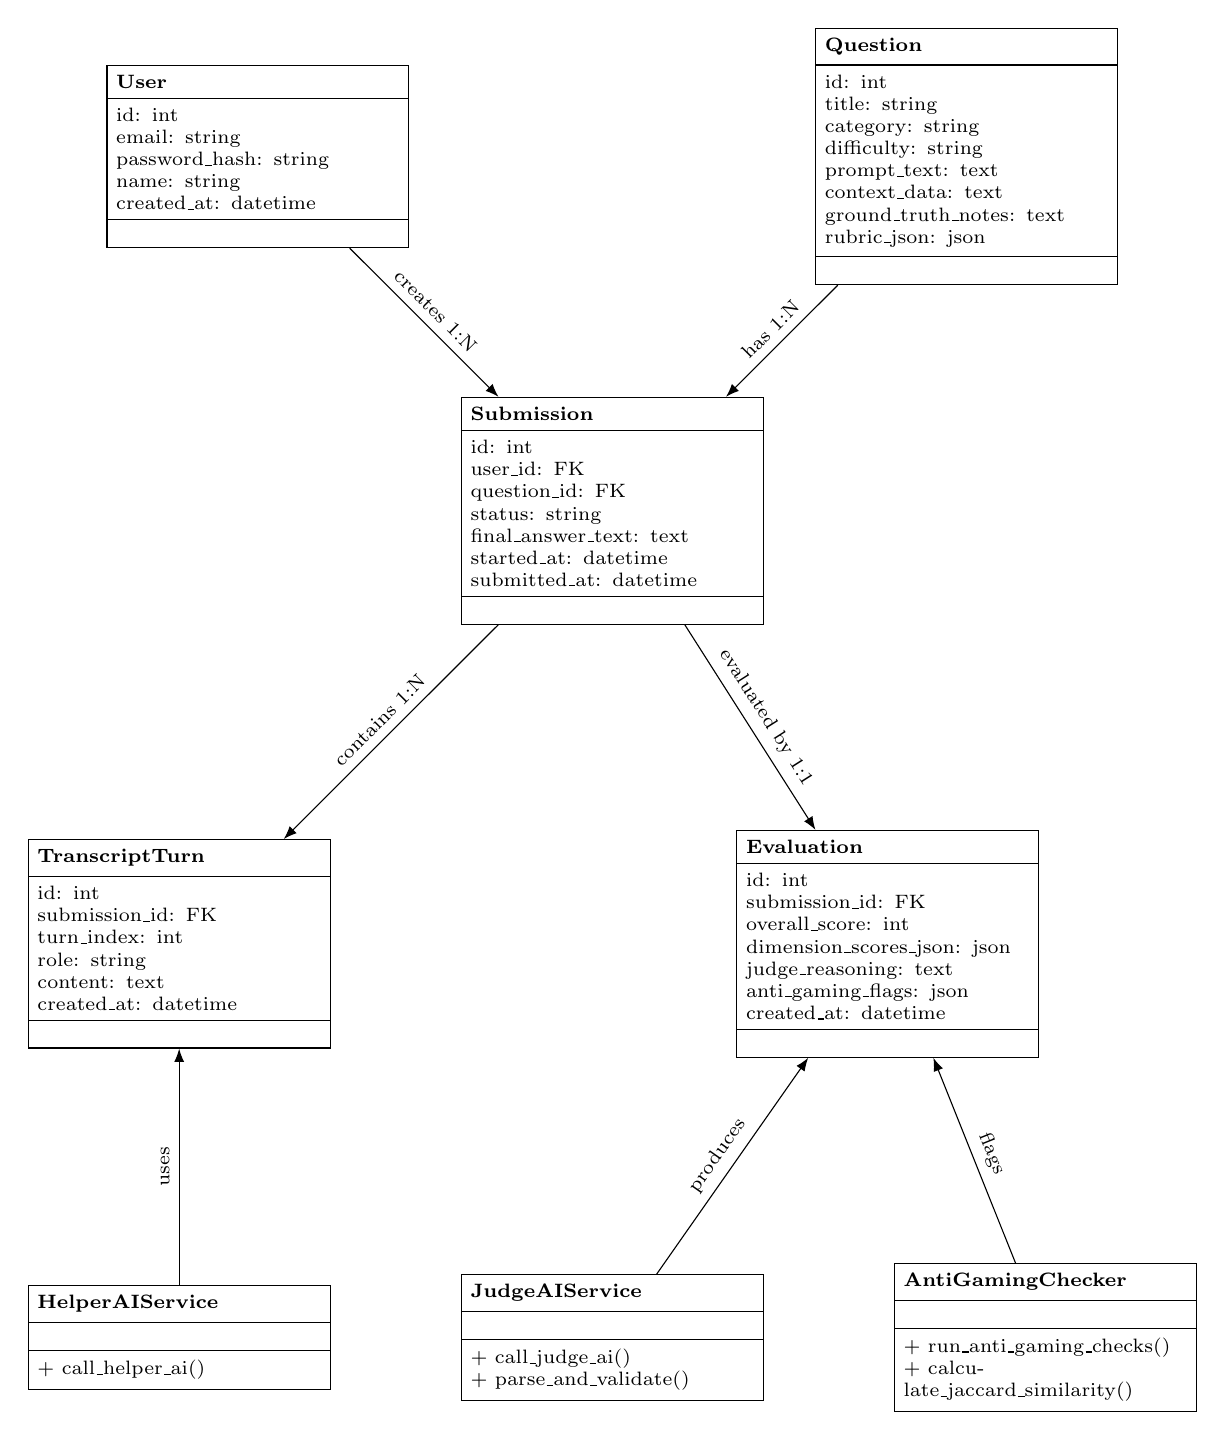
\begin{tikzpicture}[
    cls/.style={draw, align=left, font=\scriptsize, rectangle split, rectangle split parts=3, rectangle split part align={left,left,left}, text width=3.6cm}
]
\node[cls] (user) at (0,6.5) {
    \textbf{User}
    \nodepart{second} id: int\\ email: string\\ password\_hash: string\\ name: string\\ created\_at: datetime
    \nodepart{third} \phantom{x}
};

\node[cls] (question) at (9,6.5) {
    \textbf{Question}
    \nodepart{second} id: int\\ title: string\\ category: string\\ difficulty: string\\ prompt\_text: text\\ context\_data: text\\ ground\_truth\_notes: text\\ rubric\_json: json
    \nodepart{third} \phantom{x}
};

\node[cls] (submission) at (4.5,2) {
    \textbf{Submission}
    \nodepart{second} id: int\\ user\_id: FK\\ question\_id: FK\\ status: string\\ final\_answer\_text: text\\ started\_at: datetime\\ submitted\_at: datetime
    \nodepart{third} \phantom{x}
};

\node[cls] (turn) at (-1,-3.5) {
    \textbf{TranscriptTurn}
    \nodepart{second} id: int\\ submission\_id: FK\\ turn\_index: int\\ role: string\\ content: text\\ created\_at: datetime
    \nodepart{third} \phantom{x}
};

\node[cls] (eval) at (8,-3.5) {
    \textbf{Evaluation}
    \nodepart{second} id: int\\ submission\_id: FK\\ overall\_score: int\\ dimension\_scores\_json: json\\ judge\_reasoning: text\\ anti\_gaming\_flags: json\\ created\_at: datetime
    \nodepart{third} \phantom{x}
};

\node[cls] (helper) at (-1,-8.5) {
    \textbf{HelperAIService}
    \nodepart{second} \phantom{x}
    \nodepart{third} + call\_helper\_ai()
};

\node[cls] (judge) at (4.5,-8.5) {
    \textbf{JudgeAIService}
    \nodepart{second} \phantom{x}
    \nodepart{third} + call\_judge\_ai()\\ + parse\_and\_validate()
};

\node[cls] (anti) at (10,-8.5) {
    \textbf{AntiGamingChecker}
    \nodepart{second} \phantom{x}
    \nodepart{third} + run\_anti\_gaming\_checks()\\ + calculate\_jaccard\_similarity()
};

\draw[-{Latex}] (user) -- node[midway,above,sloped,font=\scriptsize] {creates 1:N} (submission);
\draw[-{Latex}] (question) -- node[midway,above,sloped,font=\scriptsize] {has 1:N} (submission);
\draw[-{Latex}] (submission) -- node[midway,above,sloped,font=\scriptsize] {contains 1:N} (turn);
\draw[-{Latex}] (submission) -- node[midway,above,sloped,font=\scriptsize] {evaluated by 1:1} (eval);
\draw[-{Latex}] (helper) -- node[midway,above,sloped,font=\scriptsize] {uses} (turn);
\draw[-{Latex}] (judge) -- node[midway,above,sloped,font=\scriptsize] {produces} (eval);
\draw[-{Latex}] (anti) -- node[midway,above,sloped,font=\scriptsize] {flags} (eval);
\end{tikzpicture}%
}
\end{center}

\section{Entity-Relationship (ER) Diagram}

The Entity-Relationship Diagram below reflects the actual PostgreSQL schema defined in
\texttt{backend/app/models.py}: a \texttt{User} creates many \texttt{Submission}s, each
\texttt{Submission} targets one \texttt{Question}, contains many ordered \texttt{TranscriptTurn}s,
and is evaluated by exactly one \texttt{Evaluation}, which embeds a \texttt{DIMENSION\_SCORES}
structure (\texttt{clarifying\_questions}, \texttt{iteration\_quality},
\texttt{hallucination\_catching}, \texttt{final\_answer\_quality}).

\begin{center}
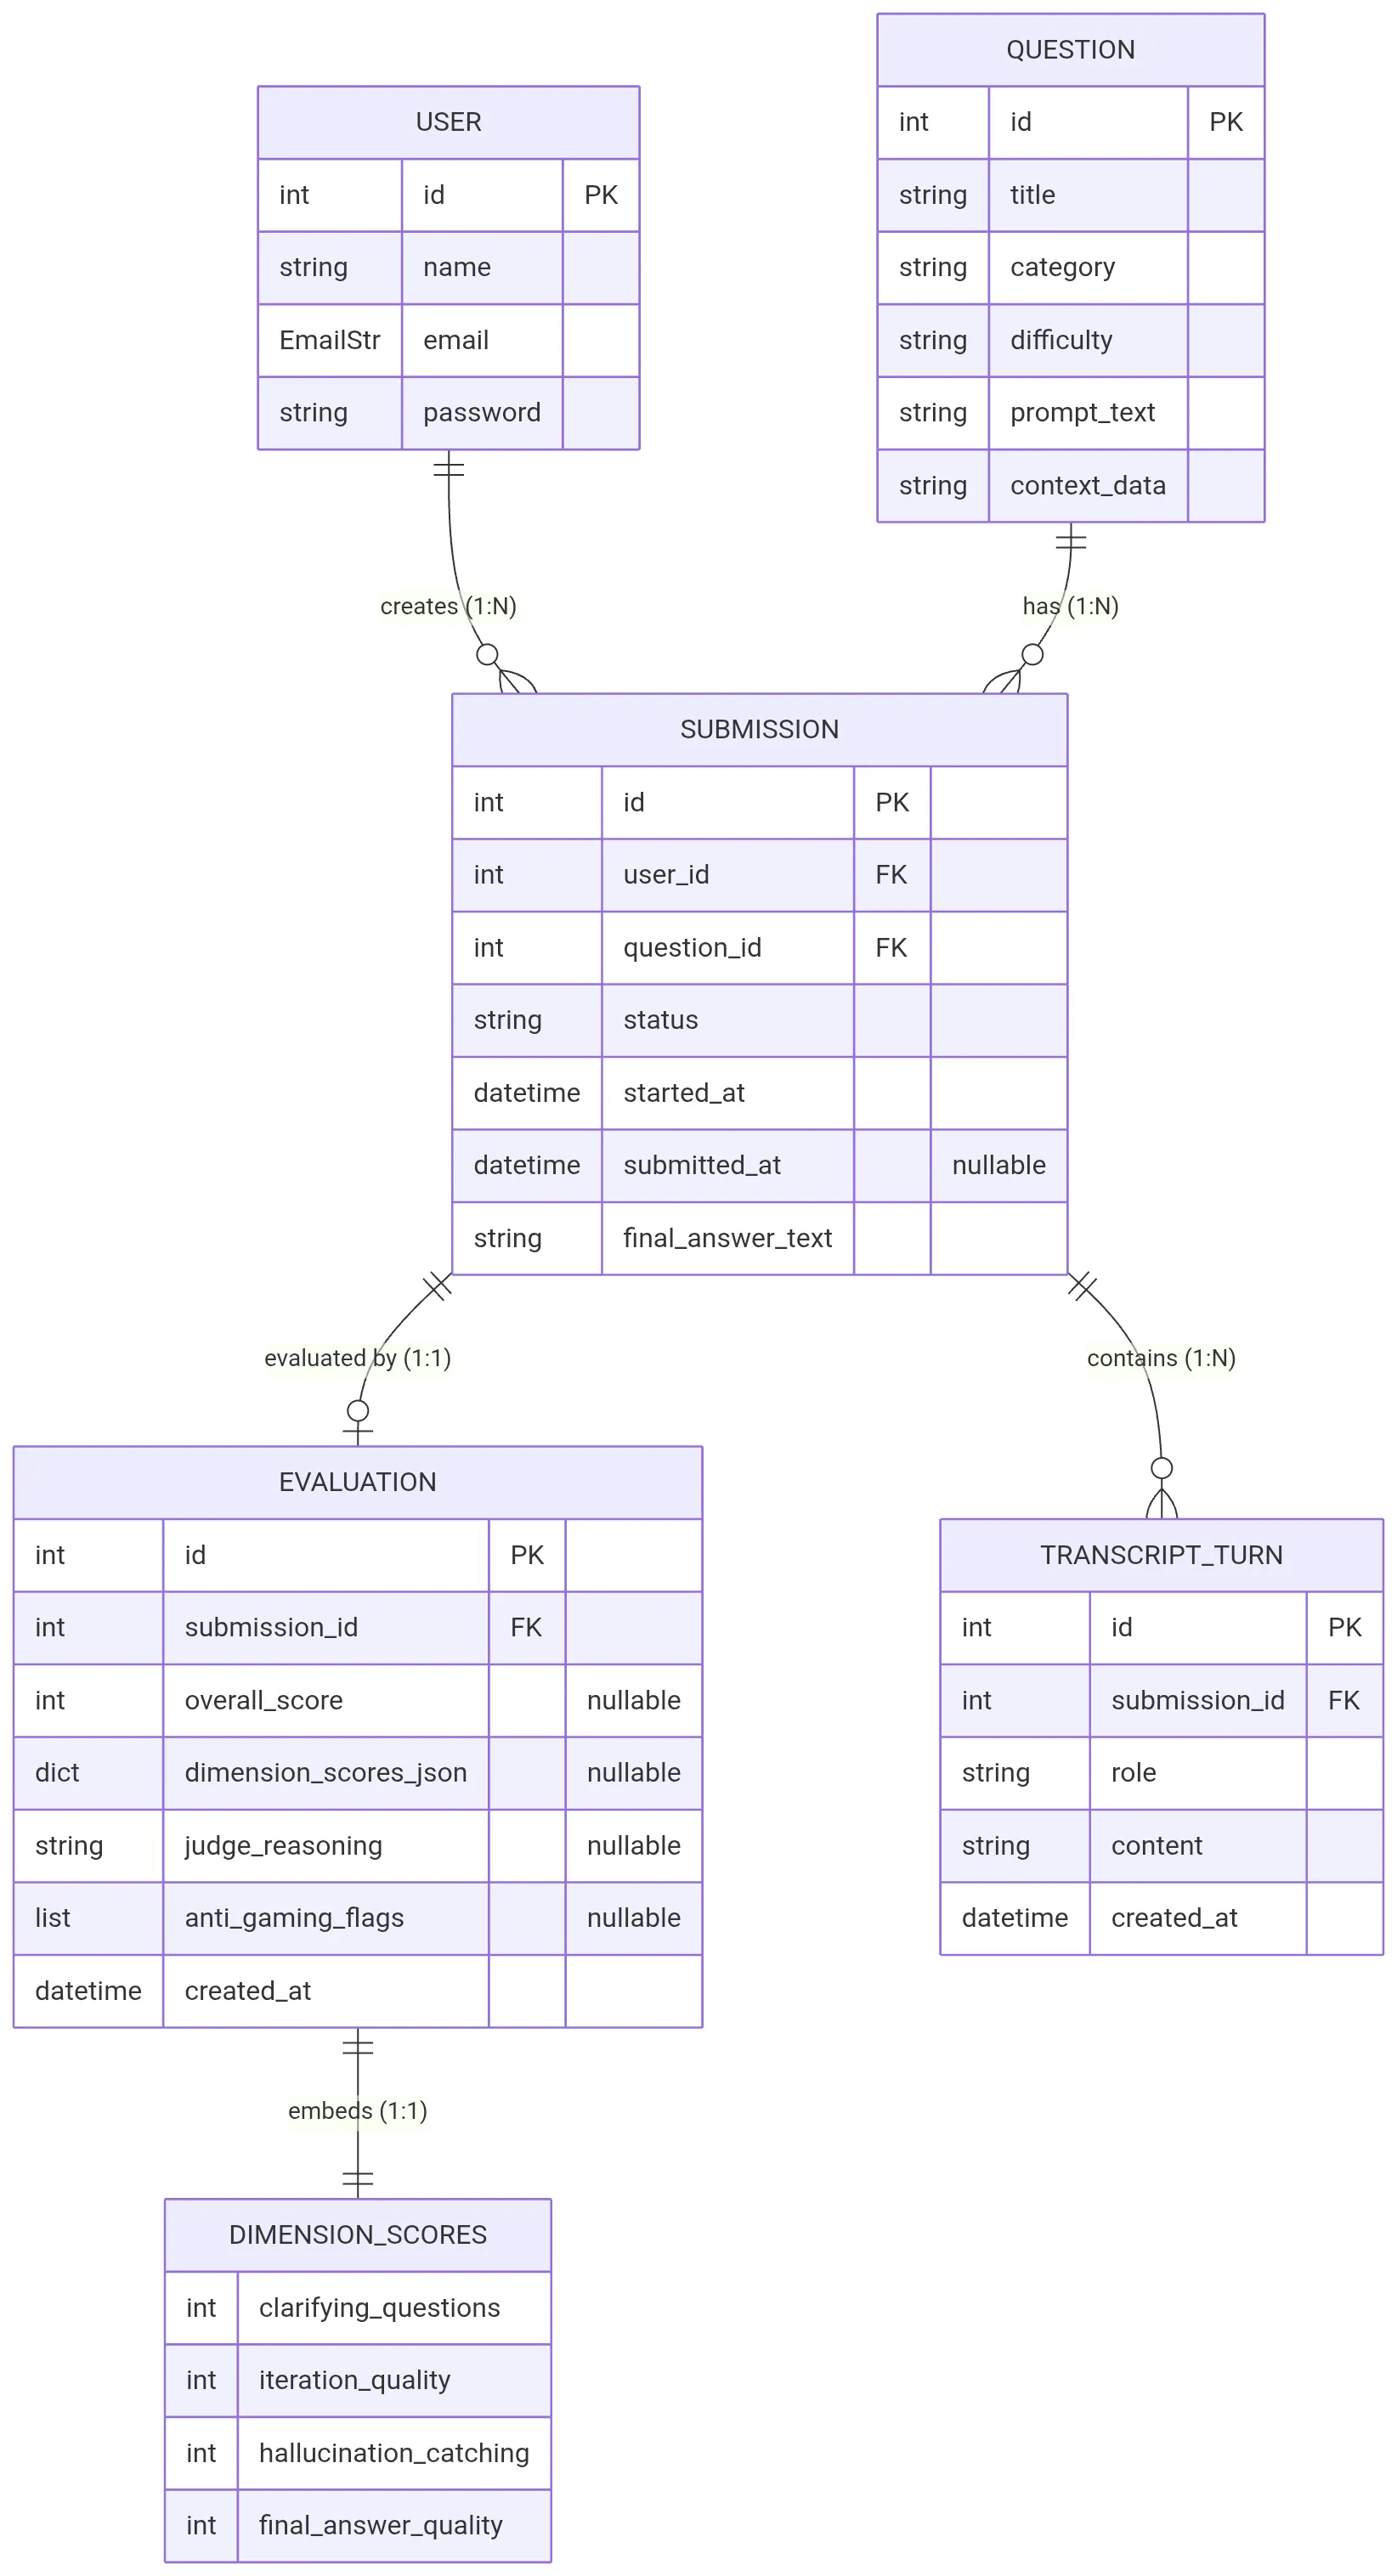
\includegraphics[width=0.82\textwidth]{images/er_diagram.png}
\end{center}

\end{document}
